%\renewcommand{\thefootnote}{\arabic{footnote}}
\chapter{TINJAUAN PUSTAKA}
\label{BAB2:tinjauan}

\section{Gas Rumah Kaca (GRK)}
Perubahan iklim telah menjadi isu keamanan internasional yang penting dan nontradisional. Emisi GRK yang berlebihan merupakan salah satu penyebab utama dari meningkatnya permasalahan iklim. Perubahan iklim tidak hanya secara langsung mempengaruhi kesehatan populasi dengan meningkatkan frekuensi dan intensitas gelombang panas, kekeringan, dan curah hujan yang tinggi, tetapi juga secara tidak langsung dengan meningkatkan polusi udara, mempercepat penyebaran vektor penyakit, serta mempengaruhi keamanan pangan dan kesehatan mental. Emisi GRK yang berlebihan menjadi faktor yang memperburuk perubahan iklim dan dampaknya terhadap berbagai aspek kehidupan manusia \cite{wang_impact_2022}.

GRK merujuk pada gas-gas yang hadir di atmosfer, baik secara alami maupun sebagai hasil aktivitas manusia (antropogenik), yang mampu menyerap dan memancarkan kembali radiasi inframerah \cite{purnamasari_inventarisasi_2019}. Ketika permukaan bumi menerima radiasi matahari dalam bentuk gelombang pendek, sebagian besar radiasi ini dipancarkan kembali ke atmosfer sebagai radiasi gelombang panjang (infra merah). GRK yang terdapat di lapisan atmosfer yang dekat dengan permukaan bumi menyerap radiasi gelombang panjang ini, menyebabkan peningkatan suhu yang tinggi yang dikenal sebagai efek rumah kaca. Peningkatan suhu ini terjadi akibat perubahan kondisi dan komposisi atmosfer yang mengelilingi planet ini \cite{pratama_efek_2019}.

Dalam era saat ini, masalah lingkungan telah menjadi pembahasan utama baik di negara-negara yang sedang berkembang maupun negara-negara maju karena adanya kerusakan lingkungan. Hal ini juga menimbulkan pertanyaan tentang pemanasan global dan perubahan iklim, yang terutama disebabkan oleh emisi GRK, kadang-kadang terkait dengan penyebab alami seperti pergeseran benua, aktivitas gunung berapi, radiasi matahari, dan arus laut, serta aktivitas manusia langsung maupun tidak langsung yang mempengaruhi komposisi atmosfer global dan variasi lingkungan \cite{li_relationship_2023}. Para peneliti telah berargumen bahwa peningkatan aktivitas manusia akibat perkembangan industrialisasi, pertumbuhan populasi global, dan kebutuhan untuk mengatasi perubahan tersebut adalah penyebab utama perubahan iklim. Selain itu, aktivitas manusia seperti deforestasi pertanian dan komersial, pembakaran bahan bakar fosil, serta perubahan penggunaan lahan akibat pertumbuhan populasi juga memberikan kontribusi yang signifikan terhadap peningkatan emisi GRK \cite{yoro_co2_2020}.

Menurut Khairunnisa Musari \& Sayah \citep{khairunnisa_musari_green_2021}, dalam rangka penyelesaian masalah GRK, beberapa hal yang perlu diperhatikan adalah upaya melawan perubahan iklim, prioritas nasional, transformasi kebijakan, menciptakan lingkungan yang mendukung, dan investasi keuangan yang diperlukan, yang semuanya harus menjadi bagian dari agenda nasional. Selain itu dengan perkembangan era informasi saat ini, salah satu upaya dengan pemanfaatan teknologi atau kecerdasan buatan (\textit{Artificial Intelligence}/AI) menjadi hal yang penting karena dapat digunakan untuk pemantauan, analisis, dan pengelolaan data terkait emisi GRK. Sementara itu, dapat membantu dalam mengoptimalkan kebijakan dan strategi untuk mengurangi emisi GRK secara efisien. Dengan memanfaatkannya secara holistik, diharapkan dapat memberikan penyelesaian masalah GRK dan perubahan iklim dapat tercapai dengan lebih efektif dan efisien.

\section{\textit{Text Mining}}
Studi literatur mengenai \textit{text mining} telah menjadi area penelitian yang semakin populer dalam ilmu data dan pengolahan bahasa alami. \textit{Text mining} merupakan teknik yang digunakan untuk mengekstraksi informasi berharga dari data teks yang tidak terstruktur, seperti artikel jurnal, berita, dan dokumen teks lainnya. Teknik ini mencakup beberapa tahapan, termasuk pengumpulan data teks, pemrosesan teks untuk menghapus karakter-karakter tidak penting, dan analisis data untuk mengidentifikasi pola, topik, atau informasi penting dari teks tersebut \cite{Salloum2018}.

Dalam penerapannya, \textit{text mining} telah digunakan dalam berbagai bidang. Misalnya, dalam analisis sentimen, \textit{text mining} dapat digunakan untuk mengekstraksi sentimen atau perasaan dari teks yang ditulis oleh pengguna dalam media sosial atau ulasan produk \cite{aqlan2019}. Selain itu, dalam pengelompokan topik, \textit{text mining} dapat membantu mengelompokkan dokumen-dokumen teks berdasarkan tema atau topik yang sama.

Dalam penelitian ini, \textit{text mining} akan digunakan sebagai salah satu teknik dalam \textit{preprocessing} \textit{dataset} berupa teks untuk mendapatkan kata kunci yang relevan dengan permasalahan GRK di Indonesia. Teknik \textit{text mining} akan membantu dalam ekstraksi fitur teks dari data teks yang tidak terstruktur, yakni abstrak dari jurnal penelitian yang terdapat pada \textit{dataset}. Proses \textit{text mining} akan melibatkan langkah-langkah seperti dengan teknik \textit{stopwords, lemmatization, punctuation, word frequency} dari ekstraksi \textit{unigram} yang akan menjadi kata-kata dasar dari \textit{dataset} tersebut.

\subsection{\textit{Natural Language Processing} (NLP)}
Bahasa Pemrosesan Alami atau yang biasa disebut \textit{Natural Language Processing} (NLP) adalah bidang keilmuan yang berfokus pada pemahaman dan penerapan bahasa manusia dalam bentuk teks atau ucapan oleh komputer. NLP telah mengalami perkembangan pesat dalam beberapa dekade terakhir, berkat kemajuan teknologi komputasi dan kemampuan mesin dalam memproses data secara lebih efektif. Salah satu tantangan utama dalam NLP adalah mengenali dan memahami struktur dan makna dari teks bahasa manusia, karena bahasa manusia seringkali ambigu dan penuh dengan variasi. Beberapa aplikasi praktis dari NLP termasuk mesin penerjemah, asisten virtual, analisis sentimen, pengenalan suara, dan masih banyak lagi. NLP telah menjadi bidang penelitian yang sangat menarik dan relevan dalam era informasi digital yang sedang berkembang pesat \cite{tiwari2023}.

Salah satu pendekatan populer dalam NLP adalah menggunakan teknik pembelajaran mesin (machine learning) untuk mengajarkan komputer bagaimana memahami dan memproses bahasa manusia. Teknik-teknik ini melibatkan penggunaan model statistik dan algoritma yang kompleks untuk mengidentifikasi pola, keterkaitan, dan makna dalam teks bahasa manusia. Contoh teknik pembelajaran mesin yang sering digunakan dalam NLP termasuk model berbasis aturan, model berbasis vektor, dan model berbasis jaringan saraf tiruan \cite{CHUNG2023105020}. Dalam beberapa tahun terakhir, penggunaan jaringan saraf tiruan, khususnya dalam bentuk transformasi bahasa seperti BERT dan GPT-3, telah mencatat kemajuan signifikan dalam banyak tugas NLP, seperti penerjemahan mesin dan pemahaman bahasa alami \cite{MOON2022104465}.

Dalam penelitian ini, teknik pemrosesan bahasa alami (Natural Language Processing/NLP) akan digunakan dalam tahapan \textit{text mining} pada data berupa teks untuk mendapatkan kata kunci yang relevan. Proses pada tahapan tersebut meliputi \textit{preprocessing} dengan menerapkan langkah-langkah seperti menghapus kata umum dan tanda baca, lematisasi, serta mendapatkan kata-kata yang relevan dari teks. Selain itu, teknik ekstraksi fitur seperti metode Term Frequency-Inverse Document Frequency (TF-IDF) digunakan untuk mengidentifikasi kata-kata yang paling penting dan mewakili konten teks secara numerik \cite{Nasimuzzaman2023}. Hasil dari penggunaan NLP dalam pemrosesan data teks ini akan digunakan sebelum menentukan hasil interpretasi yang diharapkan pada penelitian ini.

\subsection{\textit{Term Frequency-Inverse Document Frequency} (TF-IDF)}
TF-IDF (\textit{Term Frequency-Inverse Document Frequency}) merupakan salah satu teknik yang sering digunakan dalam pengolahan teks dan \textit{Information Retrieval} (IR). Teknik ini berfungsi untuk memberikan bobot pada setiap kata dalam dokumen berdasarkan frekuensi kemunculan kata tersebut dalam dokumen itu sendiri (TF) dan kebalikannya, yakni berdasarkan keberbedaan jumlah dokumen yang mengandung kata tersebut di dalam seluruh koleksi dokumen (IDF) \cite{setiawan2022feature}. Dengan menggunakan TF-IDF, kata-kata yang sering muncul dalam suatu dokumen tetapi jarang muncul di dokumen lain akan memiliki bobot yang tinggi, sehingga dapat dianggap sebagai kata kunci atau kata yang lebih penting dalam konteks dokumen tersebut. Penggunaan TF-IDF telah terbukti efektif dalam berbagai aplikasi seperti klasifikasi teks, analisis sentimen, dan sistem rekomendasi, serta telah menjadi salah satu teknik yang populer dalam mengolah teks untuk mendapatkan informasi yang bermakna \cite{sentimanaly2023}.

Adapun TF-IDF \textit{Vectorizer} adalah salah satu fungsi yang digunakan dalam pengolahan teks untuk mengimplementasikan metode TF-IDF. TF-IDF \textit{Vectorizer} berfungsi untuk mengubah teks menjadi vektor numerik berdasarkan nilai TF-IDF dari setiap kata dalam teks \cite{sentimanaly2023}. Proses ini memungkinkan data teks yang kompleks dan tidak terstruktur diubah menjadi representasi numerik yang dapat diolah lebih lanjut dengan algoritma pembelajaran mesin atau analisis statistik.

Penggunaan TF-IDF \textit{Vectorizer} sangat berguna dalam analisis teks dan NLP, terutama dalam pemrosesan data besar yang mengandung banyak dokumen atau teks. Dengan menggunakan TF-IDF \textit{Vectorizer}, dapat dilakukan suatu pengelompokan teks, analisis sentimen, deteksi topik, dan sistem rekomendasi secara efisien. Selain itu, dengan menerapkan TF-IDF \textit{Vectorizer} dalam penelitian ini mengenai emisi GRK di Indonesia, data teks abstrak akan dikonversi menjadi representasi vektor TF-IDF dengan memperhitungkan bobot kata dalam setiap abstrak. Kata-kata kunci yang relevan dalam data teks yang berkaitan dengan GRK dan menganalisis tingkat signifikansinya dalam dokumen tersebut.

\subsection{\textit{Principal Component Analysis} (PCA)}
PCA (\textit{Principal Component Analysis}) adalah sebuah metode statistik yang digunakan untuk mengurangi dimensi dari data dengan mempertahankan informasi yang paling penting. PCA digunakan untuk mengidentifikasi pola dalam data, dan mengubah data tersebut menjadi bentuk yang lebih mudah dipahami dan diinterpretasikan \cite{kurita2019principal}. 

PCA lebih sering digunakan dalam analisis data numerik, namun PCA juga dapat digunakan dalam analisis teks. Dalam analisis teks, PCA digunakan untuk mengurangi dimensi dari data teks dengan mempertahankan informasi yang paling penting \cite{beattie_exploration_2021}. PCA dapat digunakan untuk mengidentifikasi pola dalam data teks, seperti pola kata yang sering muncul bersama-sama atau pola topik yang terkait. Dengan mengurangi dimensi dari data teks, PCA dapat mempermudah analisis dan interpretasi data teks. 

\subsection{K-Means}
K-Means adalah salah satu algoritma \textit{clustering} yang paling populer digunakan dalam analisis data. Algoritma ini digunakan untuk membagi data menjadi beberapa kelompok atau klaster berdasarkan kesamaan fitur atau karakteristik tertentu \cite{jahwar2020meta}. Dalam K-Means, data dikelompokkan berdasarkan jarak antara titik data dan \textit{centroid}, yang merupakan pusat dari setiap klaster. Tujuan dari algoritma ini adalah untuk meminimalkan varians dalam setiap klaster dan memaksimalkan jarak antara klaster.

Salah satu penerapan K-Means yang sering digunakan adalah dalam analisis teks. Dalam analisis teks, K-Means digunakan untuk mengelompokkan dokumen berdasarkan kesamaan topik atau kata kunci tertentu \cite{ikotun_kmeans_2023}. Misalnya, jika kita memiliki kumpulan dokumen tentang olahraga, K-Means dapat digunakan untuk mengelompokkan dokumen berdasarkan jenis olahraga atau topik tertentu seperti sepak bola, basket, atau tenis. Dalam hal ini, K-Means dapat membantu mengidentifikasi pola dan tren dalam data teks yang besar dan kompleks.

K-Means dapat digunakan untuk memproses hasil dari analisis PCA (Principal Component Analysis). PCA adalah teknik statistik yang digunakan untuk mengurangi dimensi data dengan mempertahankan informasi yang paling penting. Setelah PCA diterapkan pada data, K-Means dapat digunakan untuk mengelompokkan data menjadi beberapa klaster berdasarkan kesamaan fitur atau karakteristik tertentu \cite{ikotun_kmeans_2023}. Hasil dari analisis K-Means dapat membantu mengidentifikasi pola dan tren dalam data yang besar dan kompleks, serta memudahkan interpretasi hasil analisis. 

\section{Teknik Kitchenham}
Teknik Kitchenham merujuk pada metode sistematis literature review (SLR) yang dikembangkan oleh Barbara Kitchenham, seorang peneliti terkemuka di bidang rekayasa perangkat lunak \cite{kitchenham_systematic_2009}. Pedoman Kitchenham untuk melakukan SLR telah menjadi sangat diakui dan sering disebut sebagai "teknik Kitchenham".

\vspace{1.5cm}
Teknik Kitchenham melibatkan proses dalam mengidentifikasi, mengevaluasi, dan mensintesis semua studi yang relevan pada pertanyaan atau topik penelitian tertentu. Proses ini meliputi pencarian yang komprehensif dan sistematis dari beberapa database dan sumber lainnya, pengembangan kriteria inklusi dan eksklusi, dan teknik analisis data untuk memastikan bahwa hasilnya dapat diandalkan dan tidak bias. Pedoman Kitchenham telah banyak diadopsi dalam penelitian rekayasa perangkat lunak dan telah berkontribusi pada pengembangan rekayasa perangkat lunak berbasis bukti (EBSE) \cite{kitchenham_systematic_2009, PIZARD2023107101}. Teknik Kitchenham telah menjadi metode standar untuk melakukan SLR dalam rekayasa perangkat lunak dan telah membantu meningkatkan kualitas dan keandalan penelitian di bidang tersebut.

Dalam konteks penggunaan teknik Kitchenham, terdapat penggunaan operator logika seperti \textit{AND}, \textit{OR}, dan \textit{NOT} dalam pencarian studi yang relevan. Operator logika tersebut digunakan untuk menggabungkan kata kunci pencarian dan memperluas atau mempersempit cakupan pencarian. Misalnya, jika ingin mencari studi yang relevan dengan topik "\textit{greenhouse gas}" dapat menggunakan operator logika AND untuk menggabungkan kata kunci "\textit{greenhouse}" dan "\textit{gas}". Dengan demikian, pencarian akan memperlihatkan studi yang hanya relevan dengan kedua kata kunci tersebut. 

Selain itu juga, penggunaan asterisk (*) dalam pencarian studi yang relevan juga dapat mencakup variasi kata yang terkait dengan akar kata tertentu. Misalnya, jika menggunakan kata kunci "\textit{communicat*}", pencarian akan mencakup studi yang menggunakan kata "\textit{communicate}", "\textit{communication}", "\textit{communicating}", dan sebagainya. Dengan menggunakan asterisk, akan dapat memperluas cakupan pencarian dan memastikan bahwa semua studi yang relevan ditemukan, terutama jika ada variasi dalam cara menyebutkan kata kunci tertentu.

\section{\textit{Luhn's Theory}}

Teori yang digagas oleh H. P. Luhn, dalam penelitiannya yaitu penciptaan otomatis abstrak literatur menggunakan mesin pemrosesan data \cite{luhn_automatic_1958}. Implementasi Luhn melibatkan analisis teks lengkap dari sebuah artikel dan pemilihan kalimat dan frasa kunci untuk membuat ringkasan singkat dari konten artikel. Mesin pemrosesan data IBM 704 digunakan untuk menghitung ukuran relatif signifikansi untuk kata dan kalimat individu, yang kemudian digunakan untuk memilih informasi paling penting untuk disertakan dalam abstrak. Implementasi ini terbukti efektif dalam menciptakan abstrak yang melayani tujuan abstrak konvensional dan dapat menghemat waktu dan usaha bagi pembaca literatur teknis.

\begin{figure}[H]
    \centering
    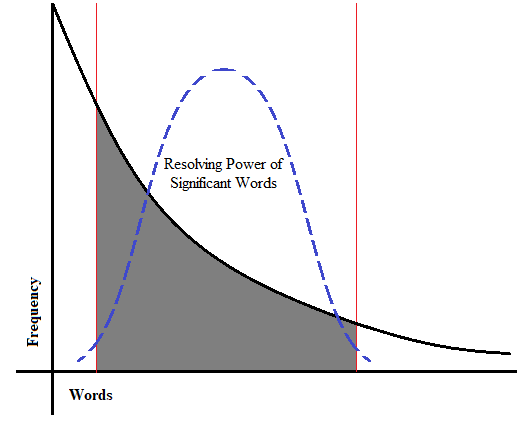
\includegraphics[width=0.6\linewidth]{img/bab2-5.png}
    \caption{Diagram \textit{Word Frequency} [8]}
    \label{fig:2-5}
\end{figure}

Hal yang menjadi sebagai kata kunci dalam penerapan metode otomatis untuk membuat abstrak literatur menggunakan mesin pemrosesan data adalah kata-kata yang paling relevan dan penting dalam artikel yang sedang dianalisis. Kata-kata ini biasanya dipilih berdasarkan topik atau subjek dari artikel tersebut. Dalam \textit{common words} seperti \textit{pronouns}, \textit{prepositions}, dan \textit{articles} dihapus dari daftar kata-kata yang dianalisis karena kata-kata ini tidak memberikan informasi yang signifikan tentang topik atau subjek dari artikel. Sebaliknya, kata-kata yang lebih spesifik dan relevan seperti kata benda dan kata kerja digunakan sebagai kata kunci untuk memilih kalimat-kalimat kunci dalam artikel yang akan digunakan untuk membuat abstrak.

Terdapat penelitian yang dilakukan oleh Rahmah et al \cite{rahmah_critical_2022} dalam menerapkan teori Luhn, dengan Hukum Zipf yang menyatakan bahwa frekuensi kemunculan sebuah kata dalam teks berbanding terbalik dengan peringkatnya dalam daftar frekuensi kata. Dalam konteks pembuatan abstrak otomatis, hukum Zipf dapat digunakan untuk memilih kata-kata kunci yang paling relevan dan penting dalam artikel yang sedang dianalisis. Selain itu, juga membahas tentang skema Bradford \cite{luhn_automatic_1958}, yang merupakan metode untuk mengelompokkan jurnal-jurnal ilmiah berdasarkan topik atau subjek yang sama, dengan adanya \textit{lower cut} dan \textit{upper cut} akan dipilih kata-kata yang diseleksi sebagai tema atau konsep yang dicari sebagaimana yang ditunjukkan pada Gambar \ref{fig:2-5} \cite{luhn_automatic_1958}. Metode tersebut digunakan untuk membantu pembaca literatur teknis menemukan jurnal-jurnal yang relevan dengan topik atau subjek yang sedang mereka teliti \cite{rahmah_critical_2022}.